\section{Introduction}\label{sec:intro}

{\em ``Over and above the actual world there are an indefinite multiplicity
of merely possible worlds... The actual world is a possible world. The other
possible worlds, the merely possible worlds, are ways that the actual world
might have been.''} \cite{Armstrong89:worlds} -- D.M. Armstrong

\vspace*{2mm}

%Traditional concurrent programs are typically subjected to blocking and race
%conditions. The exact runtime behavior is often {\em nondeterministic}
%because the actual mechanism of the (operating system) scheduler is
%{\em unknown} or too complex to the programmer {\em a priori}.
%It is easy to write a concurrent
%program that leads to deadlock or starvation -- not
%achieving termination and desired goals.

% It is essential for algorithms and programs to specify {\em choices}. 
% The most basic form of choice is a {\em conditional} or {\em if-then-else}
% construct that allows the program to execute a different control
% depending on whether a boolean condition evaluates to true or false.
% A more advanced form of choice is known as {\em nondeterminism}, which
% allows a program to specify, at certain points (called ``choice points''),
% alternative program flows. The selection of choice is not specified
% by the programmer directly, but rather by some general method applicable
% to all choice points. Nondeterminism can be thought of as a generalization of
% the conditionals. There are two existing types of nondeterminisms:
% {\em committed choice} and {\em backtracking}. Committed choice is a construct
% that contains several branches where each branch has a guard which is either
% a condition or an atomic action. The branch whose guard evaluates to true to gets
% executed first is selected over all other branches. One example of
% committed choice construct is the well known Dijstra's Guards 
% \cite{Dijkstra75:guarded}. Backtracking is an nondeterministic mechanism 
% which attempts all choice branches in some predefined sequential order 
% until some condition is found true or all choices are exhaustively searched. 
% Logic programming languages such as Prolog \cite{Lloyd87:LP}
% make extensive use of backtracking.

Concurrent programs often show non-determinism.
Furthermore, there are many important situations where
non-deterministic choices are needed in algorithms.
Programming constructs or support for non-deterministic choices 
fall into two classes:
(i) {\em don't-know non-determinism}; and (ii) {\em don't-care non-determinism}.
Don't-care non-determinism is exemplified by {\em committed choice}
such as Dijkstra's Guards \cite{Dijkstra75:guarded} and
in concurrent logic or constraint programming languages \cite{Ueda85:guarded}.
In don't-care non-determinism, although there is a choice, the selection
of which choice to execute is arbitrary (though there may be guards to restrict
availability of choices). Thus, it is the responsibility of the programmer 
to deal with the consequences of the selection.
Don't know non-determinism, on the other hand, recognizes that it might
not be possible to make the choice up front.
In a sequential language, {\em backtracking} is a typical approach.
This is typified by logic programming languages such as Prolog
which searches the combinatorial space of all possible choices to find which
choices give the desired solution. 
There are also languages which provide parallel search, i.e. some
logic programming languages give OR parallelism, but like backtracking,
it is still a search process.
When one wants to deal with problems where there is both don't know
non-determinism and concurrency, the situation can become more complex, which
is what we deal with in this paper. 
%We propose a new programming paradigm
%which is an open system with concurrent agents which can come and go and
%where speculation provides direct support for don't know non-determinism.

\begin{figure}[htb]
\centering
\epsfig{file=eps/s1flight.eps,width=0.16\textwidth}
\caption{Flight Map and Cost Between 3 Cities}\label{fig:intro-flight}
\end{figure}

The following airline ticketing scenario exemplifies our setting 
and the kind of problems where we have evolving don't know non-determinism.
Suppose a travel company $S$ sells airline tickets to its customers through an
online website, and now a traveler $T$ wants to go from $a$ to $b$. 
Such tickets are instant purchase only with a small delay to verify
and complete the transaction.
Figure \ref{fig:intro-flight} shows two possible routes,
he can fly from $a$ to $b$ (i.e. $a\to b$), 
or from $a$ to an intermediate city $c$, and then to $b$ (i.e. $a\to c\to b$).
Suppose $T$ has only \$100, and tickets $a\to b$, $a\to c$ and $c\to b$ 
cost \$100, \$50 and \$40, respectively.
%
Suppose $S$ obtains bulk tickets from airlines and puts them up for sale 
on the website dynamically, according to its own business logic. 
Customers log on and purchase tickets independently. 
So from $T$'s perspective, tickets come and go in {\em real time}. 
To secure his trip, $T$ has only two possible strategies: 
\begin{enumerate}
%\item Take a bet on one of the two routes and wait for the corresponding ticket(s). 
\item Buy the ticket which comes first, hence, committing to the 
corresponding route.
\item Try one of the route first, and if he can't get the tickets to complete
the route, try the other route.
\end{enumerate}
%
These two strategies are analogous to committed choice and backtracking
(although backtracking is extremely time limited), respectively.
In the first strategy, when $S$ sells $a\to c$ first and never sells $c\to b$, 
$T$ gets stuck after buying $a\to c$, even if $S$ puts $a\to b$ for sell later, 
as $T$ doesn't have enough money to buy both routes (only \$50 left after buying $a\to c$).
In the second strategy of $T$, there is no explicit cancellation but
there is a very short time window between selection
and actual purchase, so it is possible to abort within a short time.
However, it is unlikely, that the second strategy would lead to a different
situation than the first.
% or if it doesn't allow return of tickets at all, then $T$ can
% end up in a similar situation as the first case. 
%the ticket(s) for the selected route (either $a\to b$ or 
%$a\to c\to b$) may never appear according to the strategy of $S$.
%Then $T$ cannot acquire enough ticket(s) to fly him from $a$ to $b$.
%

\subsection{Speculation}
The previous example shows that, in many situations,
there is competition for limited resources (e.g. cash and tickets). 
The traveler can only 
attempt one of the two routes at a time. 
The drawback is of the previous strategies (committed choice or 
backtracking) are sub-optimal.
Rather than risking an incorrect choice, in this paper, we propose
a new programming model intended to avoid sub-optimal choices where possible.
In the earlier example, rather than having fixed resources, we can virtualize
them. Suppose
there are two {\em virtual} worlds, with {\em duplicated} resources.
This allows the traveler to attempt both of the routes separately and simultaneously.
One of the virtual worlds which succeeds can then be the state of the
actual resources (we discuss this further in the following sections).
We call this model of computation, {\em speculative nondeterminism}. 
It is nondeterministic because the business strategy of $S$ varies, and the traveler $T$
does not know which route will succeed, but has to execute both to find out.
It deals with concurrency since there are many users interacting with $S$.


\begin{figure}[tb]
\begin{lstlisting}[caption=Speculation. $\oplus$ denotes an exclusive choice construct.,label=lst:intro-speculate]
(wait for |$a\to b$|
 buy |$a\to b$|)
|$\oplus$|
(wait for |$a\to c$| or |$c\to b$|
 if |$a\to c$| is available
   buy |$a\to c$|; wait for |$c\to b$|; buy |$c\to b$|
 else if |$c\to b$| is available
   buy |$c\to b$|; wait for |$a\to c$|; buy |$a\to c$|)
\end{lstlisting}
\end{figure}

We now informally explain the idea of {\em speculation}.
Assume that the traveler $T$ uses speculation, i.e.
tries routes $a\to b$ and $a\to c\to b$ separately 
(see Listing \ref{lst:intro-speculate}). 
Because of the two choices by $T$, 
we create two mutually isolated environments which we call
{\em world 1} and {\em world 2} (see Figure \ref{fig:intro-speculate}). 
Each choice is mutually exclusive, for example,
in world 1, he tries route $a\to b$; whereas
in world 2, he tries route $a\to c\to b$. 
He has \$100 in each world and waits for the corresponding ticket(s).
The actions performed by $S$ are identical, so the availability of the tickets are the same.
Therefore, as long as ticket $a\to b$ (or $a\to c$ and $c\to b$) eventually comes,
$T$ can buy the ticket(s) and succeed in world 1 (or world 2).

\begin{figure}[tb]
\Tree[.$\oplus_T$
  ${\begin{matrix}
      T: a\to b \\
      (\text{world 1})
    \end{matrix}}$
  ${\begin{matrix}
      T: a\to c\to b \\
      (\text{world 2})
    \end{matrix}}$
]
\caption{Tree Structure of $T$'s Choices. $\oplus_T$ denotes the choice of $T$.}\label{fig:intro-speculate}
\end{figure}

\subsection{Exit}

Suppose there is another traveler $P$ who only wants to buy the ticket $a\to b$. 
Assume that $T$ has already create two worlds, and since $P$ has to interact
with $T$, he has to duplicate itself and execute in both worlds.
Even if $P$ gets ticket $a\to b$ before $T$ in both worlds, 
which virtual world is the {\em actual world} is still unknown
as long as $T$ is still executing his two choices. In this case,
can $P$ get out of the speculative computation with a {\em real} ticket? 
 
%?gHowever, since there will be concurrent interaction and 
%?g$P$ would also be in both worlds.
%?gWe would like to be able to exit from the virtual worlds so that
%?gone is finished with the speculative computation.
%?gSuppose 
%?gfrom the viewpoint of $S$, the state of either world is different since
%?git depends also on what happens to $T$.
% $P$ cannot leave the two worlds, because from the perspective of $S$, 
% the outcomes of the two choices from $T$ are different in this case,
% while in the reality there's only one possible outcome.
% But as $S$ is providing a long-running service, the case that 
% $P$ cannot go back to the reality with the ticket $a\to b$ is unreasonable.
% 
We provide an {\em exit} mechanism for the speculative nondeterminism framework
which allows an agent to return to the external computation outside
the virtual worlds.
Since speculation provides virtual computation in multiple worlds,
we call the exit as {\em returning to (external) reality}.
The idea is that a computation agent inside a world can
only bring out certain information which it is concerned with and
that information has to be consistent across all worlds.
For example, $P$ is only concerned about the ticket $a\to b$, 
so after $P$ possesses the ticket in both worlds, 
$P$ is allowed to leave by using exit, while 
the two worlds remain running for $S$ and $T$.
% See Section \ref{sec:language} for details of the exit mechanism. 

\subsection{Commit}

Suppose there is another traveler $Q$ who has identical choices as $T$,
and $Q$ is concerned with whether he has acquired enough tickets to go
from $a$ to $b$. 
When $Q$ speculates in the same way as $T$, 
the combination of choices from both $T$ and $Q$ 
creates 4 virtual worlds in total (see Figure \ref{fig:intro-commit}).
Assume that $S$ sells only the ticket $a\to b$ now, and
$Q$ takes the ticket in both worlds $w_1$ and $w_3$ but
$Q$'s computation in worlds $w_2$ and $w_4$ is blocked waiting for ticket
$c\to b$.
$Q$ cannot leave the speculation by using exit as it does not have the same ticket in all worlds.

\begin{figure}[thb]
\subfigure[Combination of $T$ and $Q$]{\label{fig:intro-commit}
\centering
\Tree[.$\oplus_T$
  [.${\begin{matrix}
        T: ab \\
        \oplus_Q
      \end{matrix}}$
    ${\begin{matrix}
        Q: ab \\
        (w_1)
      \end{matrix}}$
    ${\begin{matrix}
        Q: acb \\
        (w_2)
      \end{matrix}}$
  ]
  [.${\begin{matrix}
        T: acb \\
        \oplus_Q
      \end{matrix}}$
    ${\begin{matrix}
        Q: ab \\
        (w_3)
      \end{matrix}}$
    ${\begin{matrix}
        Q: acb \\
        (w_4)
      \end{matrix}}$
  ]
]}\quad
\subfigure[After Commit]{\label{fig:intro-after-commit}
\centering
\Tree[.${\begin{matrix}\vspace{6mm}\\\oplus_T\end{matrix}}$
  ${\begin{matrix}
      T: ab \\
      Q: ab ~\checkmark \\
      (w_1)
    \end{matrix}}$
  ${\begin{matrix}
      T: acb \\
      Q: ab ~\checkmark \\
      (w_3)
    \end{matrix}}$
]}
\caption{$ab$ denotes the route $a\to b$ while $acb$ denotes $a\to c\to b$. Check mark ($\checkmark$) indicates the choice works.}
\end{figure}

If some worlds are pruned, that this can make it easier for an agent to exit
as there are fewer worlds which need to be consistent. 
To prune the worlds, we introduce the {\em commit} operator
($\cm$) as shown in Listing \ref{lst:intro-commit}. 

\begin{figure}[tb]
\begin{lstlisting}[caption=Commit. $\cm$ is the commit operator. Omitted lines are the same as in Listing \ref{lst:intro-speculate}.,label=lst:intro-commit]
(wait for |$a\to b$|
 buy |$a\to b$|
 |$\cm$|)
|$\oplus$|
(wait for |$a\to c$| or |$c\to b$|
 if |$a\to c$| is available
   |$\cdots$|
 else if |$c\to b$| is available
   |$\cdots$|
 |$\cm$|)
\end{lstlisting}
\end{figure}

By using $\cm$, it indicates that the current choice works satisfactorily
and it's fine to prune the other choice. 
In the case of $Q$, once $\cm$ is reached in $w_1$ (or $w_3$), 
$w_2$ (or $w_4$) will be pruned. 
After both $w_2$ and $w_4$ are pruned, 
the tree of worlds is shown in Figure \ref{fig:intro-after-commit}.
%
%?g\begin{figure}[tb]
%?g\Tree[.$\oplus_T$
%?g  ${\begin{matrix}
%?g      T: ab \\
%?g      Q: ab ~\checkmark \\
%?g      (w_1)
%?g    \end{matrix}}$
%?g  ${\begin{matrix}
%?g      T: acb \\
%?g      Q: ab ~\checkmark \\
%?g      (w_3)
%?g    \end{matrix}}$
%?g]
%?g\caption{Tree Structure after Commit. Check mark ($\checkmark$) indicates the choice works.}\label{fig:intro-after-commit}
%?g\end{figure}
%
Now what $Q$ concerns is consistent in $w_1$ and $w_3$, 
so $Q$ can exit from the virtual worlds.

\begin{figure}[tb]
\begin{lstlisting}[caption=Preference. Omitted lines are the same as in Listing \ref{lst:intro-commit}.,label=lst:intro-commit-sleep]
(wait for |$a\to b$|
 buy |$a\to b$|
 sleep for 10 seconds
 |$\cm$|)
|$\oplus$|
(wait for |$a\to c$| or |$c\to b$|
 |$\cdots$|
 |$\cm$|)
\end{lstlisting}
\end{figure}

$\cm$ not only helps the agent exit early, 
but also can be used together with sequential constructs 
to gain more programmability. 
For instance, consider Listing \ref{lst:intro-commit-sleep},
when used together with sleep, 
the agent program can achieve some {\em preference} of 
cheaper multi-hop tickets ($a\to c\to b$ costs \$90)
over more expensive single ticket ($a\to b$ costs \$100), 
because after the traveler possesses $a\to b$ in one world, 
during the time he is sleeping, 
he may be able to acquire both $a\to c$ and $c\to b$ 
in the other world, and commit in that world to prune the sleeping one. 

\vspace*{2mm}

%\RY{shortened some text for now}

Multiple worlds was proposed in \cite{JaffarYZ07} using a
generalized committed choice (GCC) construct.
%
% informal operational semantics. GCC allows speculation between agents in 
% isolated virtual worlds. Obviously, the number of virtual worlds can 
% become exponential in the number of agents. 
% To control the explosion of worlds, 
% the {\em commit} operator was introduced,
% which can remove some unwanted choices and worlds. 
% While this allows some system resources to be reclaimed,
% it may also lead to the loss of some solutions as the commit prunes away 
% parts of the solution space.
% 
% Programming nondeterminism \cite{Floyd67} is not new. But previous 
% concurrent models restricted themselves to early
% committed choice \cite{Shapiro89:CLP-survey} or backtracking.
% We argue that maintaining combinatorial worlds 
% instead of early commits or backtracking \cite{DantsinEGV01}
% is not only good because system can explore many possibilities so that it is
% more likely to achieve the desired solution,
% but also necessary since in open and real time applications, agents
% interact with their environment autonomously and there is no global control
% over or even knowledge about the other agents. 
% 
In this paper, we generalize and extend GCC and
propose a programmable concurrency control framework called 
{\em speculative nondeterminism}, which allows concurrent agents to
\begin{itemize}
\item {\em speculate} by specifying exclusive choices and executing these
choices in combinatorial and mutually exclusive runtime environments called
worlds;
\item {\em exit} from the virtual worlds and return to reality even when
other agents are still speculating; and
\item control usage of system resources resulting from the choices
using {\em commit} operators anywhere in the program.
\end{itemize}
Our framework provides a more practical realization of speculation than GCC.
%
%Our framework is more comprehensive than GCC with a semantics that
%is geared towards more practical implementation as well as being simpler.
%It deals with the case of what happens when the agent exits the system
%and general data stores. More importantly, we show an prototype implementation
%which shows that speculative nondeterminism is practical on realistic
%examples which exploit speculation.
%
%Since commit operation has the effect of pruning some of the
%unwanted worlds, where to put the commit operator in a GCC program can have
%significant impact on the computation space. An analogy of this is the cut (!)
%predicate \cite{Billaud90:cut} in logic programming language Prolog, 
%which limits the scope of backtracking.
%Furthermore, the runtime behavior of the commit is determined by the commit semantics
%which ranges from eager to conservative. Eager commit tends to prune worlds more
%aggressively and early, while convervative commit only starts pruning when the system
%is more certain about the success of a particular choice.
% 
% Because of the combinatorial nature of the runtime system, every agent program,
% even one without any choices, is duplicated and run in multiple worlds. When
% a program runs to completion in one world, it cannot return to the main program
% immediately because other agents have not finished and there's no guarantee the world
% in which it completes will become the final reality. As such, we design a set of
% exit semantics to exactly describe the condition under which an agent can
% return to its host program without waiting for all other agents to terminate.
% This aims at improving the responsiveness of the program and thus the 
% efficency of the host program.
% 
%
This paper has two main contributions:
\begin{enumerate}
\item We propose and {\em formalize} a concurrency framework that 
exploits combinatorial choices to improve the chances of success
by agents in open and real-time applications.

The formal definition allows us to {\em precisely}
describe the operational semantics and reason about the properties and
design choices in this framework.
Moreover, the operational semantics is designed with practical
implementability in mind.
\item We have {\em implemented} a proof-of-concept prototype system 
based on the framework showing
that the system can effectively prune the 
computation space while achieving solutions in reasonable time.
\end{enumerate}

The rest of this paper is structured as follows.
Section \ref{sec:language} proposes a language for speculation
with a concrete operational semantics.
Section \ref{sec:impl} describes a runtime system we
built for the framework, and 
Section \ref{sec:experiment} evaluates the system using
three benchmarks.
Section \ref{sec:related} discusses related work and
Section \ref{sec:conclusion} concludes the paper.
